\documentclass{report}

\author{Nikhil Verma}
\usepackage{tikz}
\usepackage{amsfonts}
\usepackage{geometry}
\usepackage{ifthen}
\geometry{
    a2paper
}
\usetikzlibrary{trees}

\def\rpsarray{r/{p/{s,r}, s/{r,p}}, p/{s/{r,p}, r/{p,s}}, s/{r/{p,s}, p/{s,r}}}

% See https://tikz.dev/tikz-trees
% See https://latexdraw.com/draw-trees-in-tikz/

% Things that didn't work
% \pgfmathparse{\rpsarray[\xi]}\pgfmathresult
% \pgfmathsetmacro{\rps}{\rpsarray[\xi]}
% \pgfmathtruncatemacro{\rps}{\rpsarray[\xi]}


\begin{document}

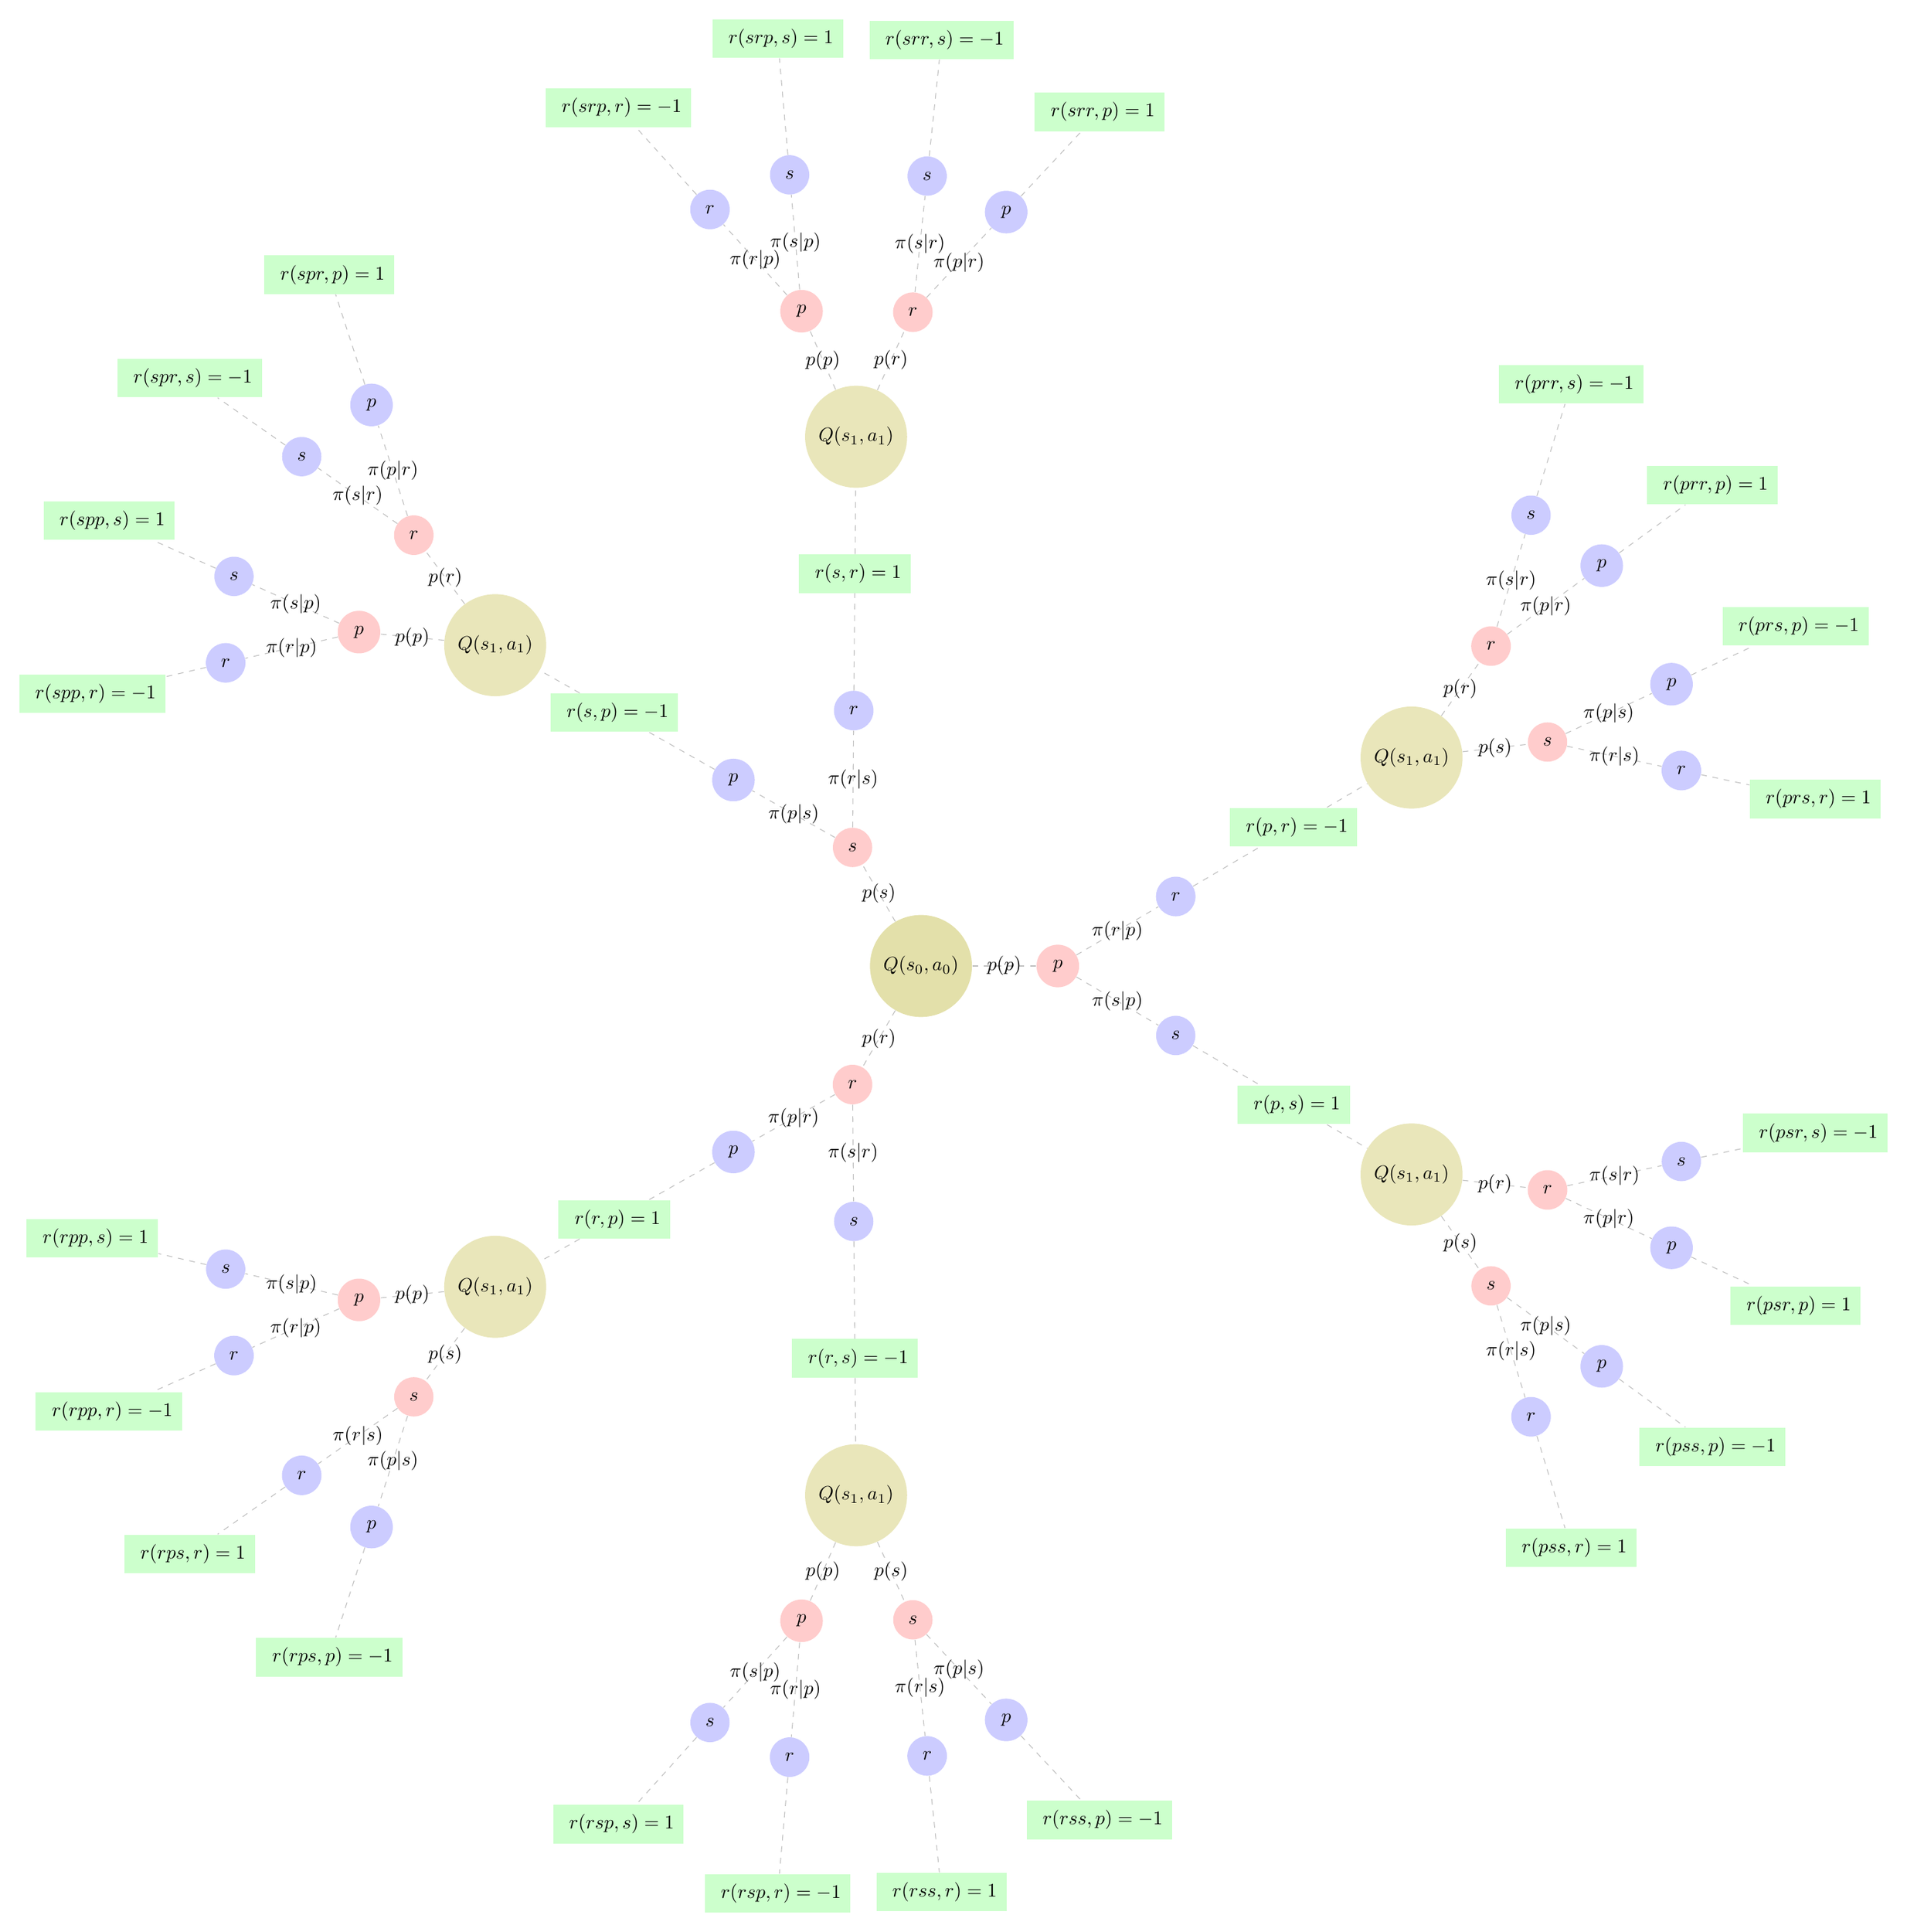
\begin{tikzpicture}
	[
        grow cyclic,
        % styles
        prob/.style = {opacity = 1},
        state/.style = {circle, fill = red!20},
        action/.style = {circle, fill = blue!20},
        reward/.style = {rectangle, fill = green!20},
        exp/.style = {circle, fill = olive!20},
        % defaults
        edge from parent/.style = {draw, dashed, opacity = 0.25},
        every node/.style = {opacity = 1, inner sep = 5pt},
        % levels
		level 1/.style = {sibling angle = 120, level distance = 2.5cm},
		level 2/.style = {sibling angle = 075, level distance = 2.5cm},
		level 3/.style = {sibling angle = 000, level distance = 2.5cm},
		level 5/.style = {sibling angle = 060, level distance = 2.5cm},
		level 6/.style = {sibling angle = 045, level distance = 2.5cm},
		% edge from parent path = {(\tikzparentnode\tikzparentanchor) .. controls +(0,-1) and +(0,1) .. (\tikzchildnode\tikzchildanchor)}
	]
	\coordinate node [circle, inner sep = 5pt, fill = olive!25] {$Q(s_0, a_0)$}
	child foreach \a/\lb [expand list = true] in \rpsarray {
    node [state] {$\a$} {
        child foreach \b/\lc [expand list = true, count = \bi from 0] in {\lb} {
        node [action] {$\b$} {
            child {
            node [reward] {\pgfmathtruncatemacro{\br}{(-1)^\bi}  $r(\a, \b) = \br$}
                child {
                node [exp] {$Q(s_1, a_1)$}
                    child foreach \c/\lc [expand list = true] in {\lb} {
                    node [state] {$\c$} {
                        child foreach \d [expand list = true, count = \di from 0] in {\lc} {
                        node [action] {$\d$} {
                            child {
                            node [reward] {\pgfmathtruncatemacro{\dr}{(-1)^\di} $r(\a\b\c, \d) = \dr$}
                            }
                        } edge from parent node [prob] {$\pi(\d|\c)$}
                        }
                    } edge from parent node [prob] {$p(\c)$}
                    }
                }
            }
        } edge from parent node [prob] {$\pi(\b|\a)$}
        }
    } edge from parent node [prob] {$p(\a)$}
    };
\end{tikzpicture}

\end{document}